\clearpage
\subsection{Global Interpolation solving}

The next step is to solve the simulation using other methods that will allow us to compare 
implementations that perform matrix-vector operations to matrix-matrix operations.
The choice is to solve the equation using a Global Interpolation based on Lagrange polynomials, The Code used is listed below and performs matrix-matrix operations to solve the problem: 


\begin{lstlisting}[language=Julia]
#using Pkg
#Pkg.add("Plots")
#Pkg.add("Kronecker")
using LinearAlgebra, SparseArrays, Kronecker, BenchmarkTools
using Plots

function print_matrix(m)
    for row in 1:size(m, 1)
        println(join(m[row, :], " "))
    end
end

# Parametros del problema
nx = 25  # Numero de puntos en la direccion x
ny = 25   # Numero de puntos en la direccion y
Lx = 1.0  # Longitud del dominio en la direccion x
Ly = 1.0  # Longitud del dominio en la direccion y
alpha = 0.001  # Difusividad termica
v = [0, 0.01]  # Vector de velocidad (vx, vy)
dt = 0.01  # Paso de tiempo
tfinal = 15  # Tiempo final de la simulacion
nsteps = Int(tfinal / dt)  # Numero de pasos de tiempo

# Definimos el tamano de la malla
dx = Lx / (nx - 1)
dy = Ly / (ny - 1)

# Inicializacion continua de temperaturas
function initialize_temperature(nx, ny, dx, dy)
    T = zeros(nx, ny)
    for i in 1:nx
        for j in 1:ny
            x = (i-1) * dx
            y = (j-1) * dy
            T[i,j] = exp(-(25*(x-0.5)^2 + 25*(y-0.5)^2))
            if T[i,j] < 0
                T[i,j] = 0
            end
        end
    end
    return T
end



# Funcion para aplicar las condiciones de frontera y mantener la fuente termica fija
function apply_boundary_conditions!(T, nx, ny, dx, dy)
    # Mantener la temperatura fija en los bordes
    T[1, :] .= exp(-(25*(-0.5)^2))
    T[end, :] .= exp(-(25*(0.5)^2))
    T[:, 1] .= exp(-(25*(-0.5)^2))
    T[:, end] .= exp(-(25*(0.5)^2))

    # Mantener la fuente termica fija en el centro con la condicion inicial
    # for i in 1:nx
    #     for j in 1:ny
    #         x = (i-1) * dx
    #         y = (j-1) * dy
    #         distance = sqrt((x - 0.5)^2 + (y - 0.5)^2)
    #         if distance <= 0.05
    #             #T[i,j] = exp(-(25*(x-0.5)^2 + 25*(y-0.5)^2))
    #             T[i,j] = 1
    #         end
    #     end
    # end
end



# Definimos los nodos en x e y
nodes_x = range(0, stop=Lx, length=nx)
nodes_y = range(0, stop=Ly, length=ny)



# ======================================================================================================

# Calculo de los polinomios de Lagrange para los x
function lagrange_basis(x_nodes, i, x)
    l_i = 1.0
    for j in 1:length(x_nodes)
        if j != i
            l_i *= (x - x_nodes[j]) / (x_nodes[i] - x_nodes[j])
        end
    end
    return l_i
end

# Funcion para calcular la derivada del polinomio de Lagrange
function lagrange_derivative(x_nodes, i, x)
    dl_i = 0.0
    for m in 1:length(x_nodes)
        if m != i
            term = 1.0 / (x_nodes[i] - x_nodes[m])
            for j in 1:length(x_nodes)
                if j != i && j != m
                    term *= (x - x_nodes[j]) / (x_nodes[i] - x_nodes[j])
                end
            end
            dl_i += term
        end
    end
    return dl_i
end

# Funcion para calcular la matriz de derivadas usando polinomios de Lagrange
function lagrange_derivative_matrix(x_nodes)
    n = length(x_nodes)
    D = zeros(n, n)
    for i in 1:n
        for j in 1:n
            D[i, j] = lagrange_derivative(x_nodes, j, x_nodes[i])
        end
    end
    return D
end


# Definimos los nodos en x e y
nodes_x = range(0, stop=Lx, length=nx)
nodes_y = range(0, stop=Ly, length=ny)

# Construccion de las matrices de derivadas con POLINOMIOS DE LAGRANGE
D_x = lagrange_derivative_matrix(nodes_x)
D_y = lagrange_derivative_matrix(nodes_y)

# Las matrices de segunda derivada son simplemente el producto de la matriz de primera derivada con ella misma
D2_x = D_x * D_x
D2_y = D_y * D_y

# ============================================================================================================




# Inicializamos el campo de temperatura
T = initialize_temperature(nx, ny, dx, dy)  # Convertimos T a un vector columna
T_new = similar(T)

# Lista para almacenar los estados de la temperatura
temperaturas = []


# Medir el tiempo del bucle
@elapsed begin
    for step in 1:nsteps

        # difusion = alpha * (Laplacian * T)
        # adveccion = -(Gradient * T)

        T_new = T .+ dt .* (alpha * (D2_x * T + T * D2_y') - (v[1] * (D_x * T) + v[2] * (T * D_y')))
        
        global T = T_new
        apply_boundary_conditions!(T, nx, ny, dx, dy)
        push!(temperaturas, copy(T))  # Guardamos el estado actual de la temperatura
    end
end


## === REPRESENTACION GRAFICA === ##

# Convertimos el resultado a una matriz para mostrarlo
T = reshape(T, nx, ny)

# Determinamos los limites de los ejes
x = range(0, stop=Lx, length=nx)
y = range(0, stop=Ly, length=ny)
z_min, z_max = 0, 1.0  # Limites del eje z (temperatura)

# # Creamos la animacion 3D
# intervalo_animacion = 30
# animation = @animate for i in 1:intervalo_animacion:length(temperaturas)
#     t = temperaturas[i]
#     surface(x, y, reshape(t, nx, ny), title="Distribucion de temperatura [M][M]", xlabel="x", ylabel="y", zlabel="Temperatura", c=:inferno, xlims=(0, Lx), ylims=(0, Ly), zlims=(z_min, z_max))
# end

# # Guardamos la animacion como un gif
# gif(animation, "adveccion_difusion_diferencias_finitas_matxmat_3d.gif", fps=30)


# Creamos la animacion 2D con lineas de contorno sin letras
intervalo_animacion = 30
animation = @animate for i in 1:intervalo_animacion:length(temperaturas)
    t = temperaturas[i]
    contourf(x, y, reshape(t, nx, ny), c=:inferno, xlims=(0, Lx), ylims=(0, Ly), zlims=(z_min, z_max), xlabel="", ylabel="", title="", clabels=false)
end

# Guardamos la animacion como un gif
gif(animation, "adveccion_difusion_contornos2d.gif", fps=10)
\end{lstlisting}

Now with a matrix-vector approach:



\subsubsection*{1. Heat Diffusion}
The heat diffusion equation describes how heat spreads through the medium over time due to thermal diffusivity. Mathematically, it is expressed as:

\[
\frac{\partial T}{\partial t} = \alpha \left( \frac{\partial^2 T}{\partial x^2} + \frac{\partial^2 T}{\partial y^2} \right)
\]

where:
\begin{itemize}
    \item \( T(x, y, t) \) is the temperature field,
    \item \( \alpha \) is the thermal diffusivity, which determines the rate at which heat diffuses through the material,
    \item \( \frac{\partial^2 T}{\partial x^2} \) and \( \frac{\partial^2 T}{\partial y^2} \) are second-order spatial derivatives representing the diffusion of heat in the \( x \) and \( y \) directions.
\end{itemize}

In this simulation, the diffusion term is discretized using \textbf{Lagrange polynomial interpolation} to approximate the second-order derivatives in both directions.
\newpage
\subsubsection*{2. Advection}
Advection describes the transport of heat due to fluid motion, which can be represented as:

\[
-\mathbf{v} \cdot \nabla T = -v_x \frac{\partial T}{\partial x} - v_y \frac{\partial T}{\partial y}
\]

where:
\begin{itemize}
    \item \( \mathbf{v} = (v_x, v_y) \) is the velocity field, representing the movement of the heat due to fluid flow,
    \item \( \nabla T \) is the gradient of the temperature, representing the directional change in temperature.
\end{itemize}

In this simulation, the velocity vector \( \mathbf{v} = [0, 0.01] \) causes heat to be advected primarily in the \( y \)-direction (upward).

\subsubsection*{3. Initial and Boundary Conditions}
\begin{itemize}
    \item \textbf{Initial Condition:} The temperature field is initialized with a Gaussian-like heat distribution centered at the middle of the domain. This represents a concentrated heat source that spreads out over time.
    \item \textbf{Boundary Conditions:} The domain has fixed temperature values at its boundaries (Dirichlet conditions). These remain constant throughout the simulation, enforcing a specific temperature on the edges of the domain.
\end{itemize}

\subsubsection*{4. Numerical Method}
The simulation uses \textbf{Lagrange polynomials} to discretize the spatial derivatives in both the \( x \)- and \( y \)-directions. This allows us to approximate the spatial derivatives necessary for solving the heat equation. 

At each time step, the temperature field is updated using the following equation:

\[
T_{\text{new}} = T + \Delta t \left( \alpha \left( \frac{\partial^2 T}{\partial x^2} + \frac{\partial^2 T}{\partial y^2} \right) - v_x \frac{\partial T}{\partial x} - v_y \frac{\partial T}{\partial y} \right)
\]

where \( \Delta t \) is the time step size, \( \alpha \) controls the rate of heat diffusion, and \( v_x \) and \( v_y \) represent the velocities in the \( x \)- and \( y \)-directions (advection).
\newpage
\subsubsection*{5. Visualization}
The simulation results are visualized as contour plots, which show the evolving temperature field over time. The animation demonstrates how the heat diffuses across the domain while being transported upward by the advection process.

\subsubsection*{Key Physical Concepts}
\begin{itemize}
    \item \textbf{Heat Diffusion:} The process by which heat spreads from areas of high temperature to low temperature.
    \item \textbf{Advection:} The transport of heat due to the fluid motion, represented by the velocity vector \( \mathbf{v} \).
    \item \textbf{Lagrange Polynomial Interpolation:} Used to discretize the spatial derivatives of the temperature field.
    \item \textbf{Boundary Conditions:} Fixed temperature values are enforced on the domain boundaries.
\end{itemize}

This combination of heat diffusion and advection captures the behavior of heat flow in systems with fluid motion and thermal effects. The numerical method used here allows for the accurate simulation of temperature evolution in the domain.

\begin{figure}[h!]
    \centering
    \begin{minipage}[b]{0.3\textwidth}
        \centering
        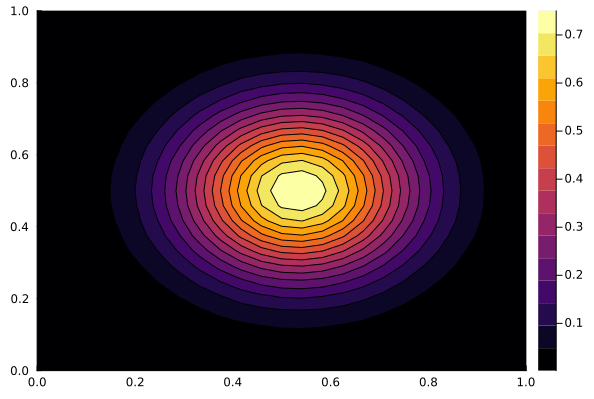
\includegraphics[width=\textwidth]{Figures/CD1.png}
        \caption{$t = 0\,\text{s}$}
    \end{minipage}
    \hfill
    \begin{minipage}[b]{0.3\textwidth}
        \centering
        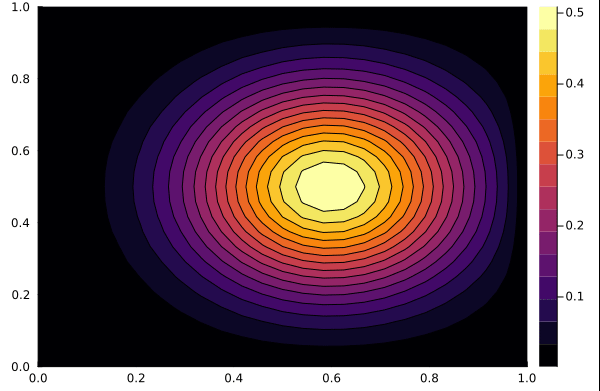
\includegraphics[width=\textwidth]{Figures/CD2.png}
        \caption{$t = 7.5\,\text{s}$}
    \end{minipage}
    \hfill
    \begin{minipage}[b]{0.3\textwidth}
        \centering
        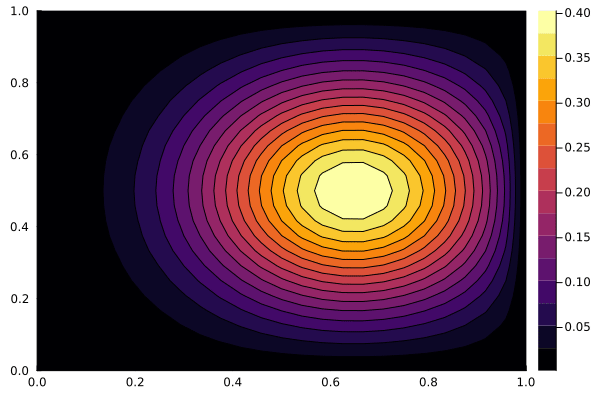
\includegraphics[width=\textwidth]{Figures/CD3.png}
        \caption{$t = 15\,\text{s}$}
    \end{minipage}
\end{figure}

